

\section{PETSc Overview}
\begin{frame}{PETSc}
   \begin{center} \Large \textbf{PETSc Overview} \end{center}
\end{frame}

\begin{frame}[fragile]
\frametitle{PETSc Origins}
 
 \begin{center} \LARGE
  \definecolor{ddviolet}{rgb}{0.561, 0.067, 0.455}  % RGB 143-17-116
  PETSc was developed as a Platform for \\[0.2em] \textbf{\color{ddviolet} Experimentation}
 \end{center}

 \vspace{1cm}
 \begin{block}{We want to experiment with different}
 \begin{itemize}
  \item Models
  \item Discretizations
  \item Solvers
  \item Algorithms
 \end{itemize}
 \end{block}

 \begin{block}{These boundaries are often blurred...}
 \end{block}

 \begin{flushright}
  \vspace*{-5cm}
  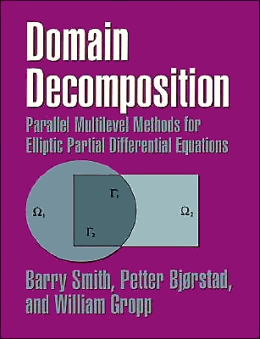
\includegraphics[width=0.4\textwidth]{dd-book-smith.png}
 \end{flushright}

\end{frame}

